\documentclass[11pt]{article}
% Arxiv
\pdfoutput=1
\usepackage[utf8]{inputenc}
\usepackage{verbatim}
\usepackage{amsmath,amssymb,array}
\usepackage{amsthm}
\usepackage{float}
\usepackage[algoruled,linesnumbered,noend]{algorithm2e}
\usepackage{ifdraft}
\usepackage{enumitem}
\usepackage{cite}
\usepackage{rotating}
\usepackage{multirow}
\usepackage{verbatim}
\usepackage{url}
\usepackage{amsthm}
\usepackage{xspace}
\usepackage{graphicx}
\usepackage{verbatim}
\newcommand{\coll}[1]{\url{#1}}

% REMOVE BEFORE SUBMISSION - begin part
\usepackage{verbatim}
\newcommand{\nota}[1]{%
  {\sffamily\bfseries #1}%
  \marginpar{\framebox{\Large *}}%
}
\newcommand{\notaestesa}[2]{%
  {\sffamily {\bfseries #1}{\footnotesize #2}}%
  \marginpar{\framebox{\Large *}}%
}

\usepackage{tikz}
\usetikzlibrary{shapes,arrows}
\usetikzlibrary{snakes}
\usetikzlibrary{positioning,patterns}
\usepackage{subfigure}

\usepackage{rotating}



\newcommand{\mathfrc}[1]{\text{\fontfamily{frc}\selectfont#1}}



\usepackage{booktabs}
\newcommand{\otoprule}{\midrule[\heavyrulewidth]}
\newcommand{\lmidrule}{\midrule[.4\heavyrulewidth]}
\usepackage{tabularx}
\newcolumntype{T}[1]{>{\tsize} #1}
\newcolumntype{W}{>{\raggedleft\arraybackslash}X}
\newcolumntype{C}{>{\centering\arraybackslash}X}
\usepackage{multirow}
\usepackage{longtable}
\usepackage{array}


\newcommand{\nheader}[1]{\multicolumn{1}{c}{#1}}
\newcommand{\header}[1]{\multicolumn{1}{c}{\headsize #1}}
\newcommand{\headertwo}[1]{\multicolumn{2}{c}{\headsize #1}}
\newcommand{\notfound}{\multicolumn{8}{c}{\tsize did not complete the task}}
\newcommand{\tsize}{\scriptsize}
\newcommand{\headsize}{\scriptsize}

\newcommand{\plaintable}{%
  \setlength{\extrarowheight}{0ex}%
}
\newcommand{\plainlongtable}{%
  \setlength{\extrarowheight}{-0.45ex}%
}

\newcommand{\longtableheader}[4]{
\caption[#3]{#2}\\
\toprule #4 \otoprule
\endfirsthead
\caption[]{#3}\\
\toprule #4 \otoprule
\endhead
\midrule
\multicolumn{#1}{r}{\tsize (continue)}\\
\endfoot
\bottomrule
\endlastfoot
}

\newcommand{\inputdata}[1]{\noindent \emph{Input: }#1\\*}
\newcommand{\outputdata}[1]{\noindent \emph{Output: }#1\\}
\newcommand{\ie}{i.e.~}
\newcommand{\st}{s.t.~}
\newcommand{\wrt}{w.r.t.~}
\newcommand{\ExGene}{\ensuremath{\langle B,F\rangle}}
\newcommand{\Path}{\ensuremath{\mathcal{P}}}
\newcommand{\nil}{\ensuremath{\bot}}
\newcommand{\card}[1]{\ensuremath{|#1|}}
\DeclareMathOperator{\prefix}{pre}
\DeclareMathOperator{\suffix}{suf}
\DeclareMathOperator{\enc}{enc}
\DeclareMathOperator{\FH}{LH}
\DeclareMathOperator{\SH}{RH}
\renewcommand{\l}{\ensuremath{\ell}}
\renewcommand{\emptyset}{\ensuremath{\varnothing}}


\begin{document}

\newtheorem{theorem}{theorem}[section]
\newtheorem{lemma}[theorem]{Lemma}
\newtheorem{proposition}[theorem]{Proposition}
\newtheorem{observation}[theorem]{Observation}
\newtheorem{corollary}[theorem]{Corollary}
\newtheorem{claim}[theorem]{Claim}
\newtheorem{property}[theorem]{Property}
\theoremstyle{definition}
\newtheorem{definition}[theorem]{Definition}
\newtheorem{problem}{problem}
%\newtheorem{example}{example}[section]



\title{RNA-Seq Graph Builder Manual}
% \titlerunning{}

\author{Stefano Beretta\thanks{%
DISCo, Univ. di Milano-Bicocca, Milan, Italy email: {beretta@disco.unimib.it}}
}
%\authorrunning{S. Beretta, P. Bonizzoni, G. Della Vedova \and R. Rizzi}

% \institute{DISCo,
%   Univ. Milano-Bicocca,
%   Milan, Italy\\ \email{\{beretta,bonizzoni,rizzi\}@disco.unimib.it}
% \and Dip. Statistica, Univ. Milano-Bicocca,
%   Milan, Italy\\ \email{gianluca.dellavedova@unimib.it}
% }

\maketitle

\emph{RNA-Seq Graph Builder} is a method to reconstruct the Splicing
Graph of a gene from RNA-Seq data, without the genome information,
where such a graph is a representation of the variants of alternative
splicing of the gene structure.

This program predicts from NGS data the gene structure induced by the
different full-length isoforms due to alternative splicing. More
precisely, it analyzes RNA-Seq reads that have been sampled from the
transcripts of a gene, with the goal of building a graph
representation of the variants of alternative splicing corresponding
to those full-length isoforms. The novelty of this method relies on
the fact that it builds such a graph in absence of the genome.

\section{Download and Installation}
\emph{RNA-seq-Graph-Builder} is implemented in $C++$ and is currently
distributed only on source form. It has been developed on Ubuntu Linux
machines (v. $10.04$ and $10.10$) and has been tested on both $32$ and
$64$ bit. The program also requires the $C++$ library \emph{SEQAN}
available at \url{http://www.seqan.de} or in Ubuntu systems it is
possible to install the develop package seqan-dev by typing:
\begin{verbatim}
$ sudo apt-get install seqan-dev
\end{verbatim}

\subsection*{Download}
\emph{RNA-seq-Graph-Builder} is developed on the AlgoLab/RNA-seq-Graph Git
repository hosted by GitHub. The repository can be explored using the
GitHub web interface at \url{https://github.com/AlgoLab/RNA-seq-Graph}.

It is also possible to clone the entire repository using the following
command:
\begin{verbatim}
$ git clone git://github.com/AlgoLab/RNA-seq-Graph.git
\end{verbatim}

The source code is available directly in:
\begin{description}
\item[zip] \url{https://github.com/AlgoLab/RNA-seq-Graph/zipball/v2.0.0}
\item[tar.gz] \url{https://github.com/AlgoLab/RNA-seq-Graph/tarball/v2.0.0}
\end{description}

\subsection*{Compilation}
The program can be compiled by issuing the command at the command
prompt:
\begin{verbatim}
$ make
\end{verbatim}

\section{Usage}
The program takes as input a FASTA file with the RNA-seq data of a
gene and returns the RNA-Seq Graph. The program is executed by typing
the following command:
\begin{verbatim}
$ ./bin/build_RNA_seq_graph [options] --reads <RNA-Seq_file>
\end{verbatim}
where the possible options are:
\begin{verbatim}
-o <graphML_out_file> (Default: std output)

--ref_level {1-5}
\end{verbatim}
\begin{enumerate}
\item Standard Algorithm (Default option)
\item Add tiny blocks
\item Add linking edges
\item Add small blocks
\item Refine overlapping nodes
\end{enumerate}
A summary of the available program options can be printed by invoking:
\begin{verbatim}
$ ./bin/build_RNA_seq_graph
\end{verbatim}
without parameters, or:
\begin{verbatim}
$ ./bin/build_RNA_seq_graph --help
\end{verbatim}
Alternatively it is possible to view the debug options by typing:
\begin{verbatim}
$ ./bin/build_RNA_seq_graph --advanced
\end{verbatim}
An example of usage is:
\begin{verbatim}
$ ./bin/build_RNA_seq_graph --reads Raw_reads_file.fa -o Out_file
\end{verbatim}

\section{File Formats}
\subsection*{Input: RNA-Seq Dataset}
RNA-Seq file is in FASTA format (.fa, .fas or .fasta). In particular,
each line of the input file describes a single read and it is composed
by at least 2 rows: the first one is the header of the read (that
usually starts with '\url{>}') and the second one that contains the
sequence. For example:
\begin{verbatim}
>B2GA004:3:100:1143:752#0/1 /source=region /gene_id=gene /gene_strand=+
GATGAAATACTACTTCTACCATGGCCTTTCCTGGCCCCAGCTCTCTTACATTGCTGAGGACGAGAATGGGAAGAT
\end{verbatim}
\subsection*{Output: RNA-Seq Graph}
The program produces as output a file in txt format that contains a
list of nodes and arcs of the RNA-Seq graph. It also gives as output
the same graph in GDL format
(\url{http://www.absint.com/aisee/manual/windows/node58.html}). It also
print on standard output the graph in GraphML format; this latter can
be redirected into a file in order to visualize or export it. By
default the files are \emph{RNA-seq-graph.txt} and \emph{RNA-seq-graph.gdl}. For
example:
\begin{verbatim}
$ ./bin/build_RNA_seq_graph --reads Raw_file.fa > RNA-seq-graph.graphml
\end{verbatim}
If the option \url{-o} is specified the 3 files will have the specified name:
\begin{verbatim}
$ ./bin/build_RNA_seq_graph --reads Raw_reads_file.fa -o Out-file
\end{verbatim}
generates \emph{Out-file.txt}, \emph{Out-file.gdl} and
\emph{Out-file.graphml}.

\section{Program Code Description}

\subsection*{Files}
The program is written in C++ and it is organized in the following set of files:
\begin{description}
\item[Main]: is the ``main'' method and contains the initial
menu (with the debugging options). In this file all the procedures in
the pipeline of the (standard) algorithm are called.
\item[read\_fasta]: is the file containing the procedures for building
the \emph{hash table} that index the reads. The function
\textbf{read\_fasta()} parses the RNA-Seq reads file, creates the
entry and insets them into the table.
\item[build\_chains]: in this file there are all the procedures for
the creation of the chains by using the unspliced reads (i.e. vertices
of the graph). There are also the functions to print the built chains
(used in debug mode) and to print the reads (in different ways:
left/right table, unspliced/spliced/perfectly spliced reads) in the
\emph{hash table}. The function \textbf{build\_unspliced\_chains()} is
invoked as second step of the (standard) algorithm in order to build
chains by overlapping half unspliced reads. After that, the procedure
\textbf{merge\_unspliced\_chains()} try to ``fuse'' chains that
overlaps each other (by using the \emph{hash table}.
\item[join\_chains]: in this file there are the procedures for the
creation of the links among chains by using perfectly spliced reads
(i.e. arcs of the graph). The function
\textbf{link\_fragment\_chains()} creates those links and finally
\textbf{print\_graph()} creates the graph in output in different
formats. In this file there also the following procedures:
\begin{itemize}
\item \textbf{check\_cutted\_frags()}: try to look if the fragments
cut from the chains in the linking phase can be added as graph
vertices.
\item \textbf{confirm\_links()}: adds the ``weight'' to the perfectly
spliced reads by summing the frequencies of the spliced reads that
identify the ``same junction''.
\item \textbf{gap\_linking()}: try to add further links by considering
a possible ``gap'' in the junction.
\end{itemize}
\end{description}

\subsection*{Data Structures}
The main data structures used in the program are the two hash tables
used to index the reads. In the program they are implemented as:
\begin{verbatim}
//Elements of the hash tables
struct element_table{
    table_entry* p;
    bool unspliced;
    bool half_spliced;
};

//Type of Left/Right table
typedef std::map<unsigned long long, element_table> hash_map;

//Hash tables
struct tables{
    hash_map left_map;
    hash_map right_map;
};
\end{verbatim}
In \emph{tables} there are the \emph{left\_map} and the
\emph{right\_map} hash maps that are both ``map'' of the standard
library C++ in which:
\begin{description}
\item[key] is the left (resp. right) fingerprint of the entry reads
\item[value] is an \emph{element\_table} in which there is the
concatenated list of read entry (\url{table_entry*p}) and two flags
to indicate that the entry is \emph{unspliced} or \emph{half spliced}
(i.e. perfectly spliced).
\end{description}

In figure~\ref{fig:types} a graphical representation of the types pf
the data structures is shown. In this data structures, the reads are
added to the hash tables by creating a concatenated list of
\emph{table\_entry} elements; in fact each \emph{table\_entry} element
is an instance of the class:
\begin{verbatim}
class table_entry{
    private:
    //Table List
    table_entry* r_next, r_prev;
    table_entry* l_next, l_prev;
    //Fingerprints
    unsigned long long left_fingerprint, right_fingerprint;
    //Chain List
    table_entry* chain_next, chain_prev;
    //Sequence frequency
    long frequency;
}
\end{verbatim}
in which the public set/get methods are omitted.

\begin{figure}[t]
\centering
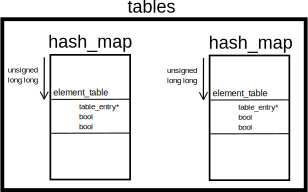
\includegraphics[scale=1.5]{img/Types}
\caption{Types of the data structures used in the program}
\label{fig:types}
\end{figure}

So by using the pointers \url{l_next} and \url{l_prev} it is possible
to build a bidirectional list of reads for the \emph{left\_map} table,
in which all those reads share the same left fingerprints (i.e. the
entry collision of the left hash table). The same \emph{table\_entry}
object is also part of the bidirectional list of the right hash table
and this is done by the two pointers \url{r_next} and \url{r_prev} for
the reads that share the same right fingerprint. So each object is
part of two list simultaneously (left and right).

The other \emph{table\_entry} pointers (\url{chain_next} and
\url{chain_prev}) are the one used in the chain composition. In
particular they link the current (unspliced) read to the (unspliced)
one that share its left fingerprint with the right fingerprint of the
current read (\url{chain_next}), and to the one that share its right
fingerprint with the left fingerprint of the current read
(\url{chain_prev}). The other values are the left and right
fingerprints of the read and the frequency (i.e. the number of
occurrences) of the read.

\section{Memory Profiling}
In order to monitor the memory consumption of the program we have used
the library for the memory profiling \url{libmemusage.so}. This
library can be preloaded using \url{LD_PRELOAD} and will intercept calls to
malloc,free,realloc and various other calls. In short it will trace
memory allocations for you:
\begin{verbatim}
$ LD_PRELOAD=/lib/libmemusage.so build_RNA_seq_graph --reads Raw_reads_file.fa
\end{verbatim}
This commando will output on \emph{std error} the memory usage of the
program on the \url{Raw_reads_file.fa} dataset. An example of the
reported output is the following: {\small
  \verbatiminput{Mem_usage_info.txt} } 

The \emph{heap peak} value indicates the maximum number of Bytes used
by the program, i.e. the memory requirement: in the previous example
it is $183838093$ Bytes, which is $\sim175$MB.

To use libmemusage all you have to do is to prepend
\url{MEMUSAGE_OUTPUT=mytrace} and \url{LD_PRELOAD=/lib/libmemusage.so}
to your application. This will instruct the library to write out a
trace to the mytrace file.

This trace file can be converted to a graph using the memusagestat
utility. It is not installed by most GNU distributions and can be
either build from the glibc sources or from the QtWebKit performance
measurement utilities. Using:
\begin{verbatim}
$ memusagestat -o output.png mytrace
\end{verbatim}
an image with memory allocations and stack usage like the one at the
end of this post will be created (i.e. \url{ouput.png}). The redline
is the heap usage, the green one is the stack usage of the
application. The x-scale is the number of allocations. The memory
occupation of the previous example is reported in
figure~\ref{fig:memusg}.

\begin{figure}[t]
%\centering
\hspace{-2cm}
\includegraphics[scale=0.6]{img/Mem_usage}
\caption{Example of memory usage output}
\label{fig:memusg}
\end{figure}

\end{document}

%%% Local Variables:
%%% mode: latex
%%% TeX-master: t
%%% TeX-PDF-mode: t
%%% ispell-local-dictionary: "english"
%%% flyspell-mode: t
%%% End:

% LocalWords:  Refseq mapping RNA-Seq isoforms unspliced struct
